\documentclass[english,onecolumn]{IEEEtran}
\usepackage[T1]{fontenc}
\usepackage[latin9]{luainputenc}
\usepackage[letterpaper]{geometry}
\geometry{verbose}
\usepackage{amsfonts}
\usepackage{babel}
\usepackage{ulem}

\usepackage{extarrows}
\usepackage[colorlinks]{hyperref}
\usepackage{listings}
\usepackage{xcolor}
\usepackage[ruled,linesnumbered]{algorithm2e}

\usepackage{amsmath,graphicx}
\usepackage{subfigure} 
\usepackage{cite}
\usepackage{amsthm,amssymb,amsfonts}
\usepackage{textcomp}
\usepackage{bm,pifont}
\usepackage{booktabs}
\usepackage{listings}
\usepackage{xparse}
\usepackage{xcolor}
\definecolor{salmon}{rgb}{1, 0.5020, 0.4471}

\NewDocumentCommand{\codeword}{v}{
\texttt{\textcolor{blue}{#1}}
}

\lstdefinestyle{mystyle}{
    backgroundcolor=\color{backcolour},   
    commentstyle=\color{codegreen},
    keywordstyle=\color{magenta},
    numberstyle=\tiny\color{codegray},
    stringstyle=\color{codepurple},
    basicstyle=\ttfamily\footnotesize,
    breakatwhitespace=false,         
    breaklines=true,                 
    captionpos=b,                    
    keepspaces=true,                 
    numbers=left,                    
    numbersep=5pt,                  
    showspaces=false,                
    showstringspaces=false,
    showtabs=false,                  
    tabsize=2
}

\lstset{style=mystyle}

\providecommand{\U}[1]{\protect\rule{.1in}{.1in}}
\topmargin            -18.0mm
\textheight           226.0mm
\oddsidemargin      -4.0mm
\textwidth            166.0mm
\def\baselinestretch{1.5}


\newtheorem{theorem}{Theorem}[section]
\newtheorem{lemma}[theorem]{Lemma}

\newcommand{\Rbb}{\mathbb{R}}
\newcommand{\Pb}{\mathbf{P}}
\newcommand{\Ib}{\mathbf{I}}
\newcommand{\vb}{\mathbf{v}}
\newcommand{\Ucal}{\mathcal{U}}
\newcommand{\Wcal}{\mathcal{W}}
\newcommand{\Vcal}{\mathcal{V}}
\newcommand{\Rcal}{\mathcal{R}}
\newcommand{\Ncal}{\mathcal{N}}
\newcommand{\bigO}{\mathcal{O}}
\newcommand{\bigS}{\mathcal{S}}
\newcommand{\bA}{{\bf A}}
\newcommand{\bQ}{{\bf Q}}
\newcommand{\bR}{{\bf R}}
\newcommand{\bH}{{\bf H}}
\newcommand{\bU}{{\bf U}}
\newcommand{\bT}{{\bf T}}
\newcommand{\bI}{{\bf I}}
\newcommand{\bq}{{\bf q}}
\newcommand{\bz}{{\bf z}}
\newcommand{\bL}{{\bf L}}
\newcommand{\bx}{{\bf x}}
\newcommand{\bv}{{\bf v}}
\newcommand{\bG}{{\bf G}}
\def\A{\mathbf{A}}
\def\v{\mathbf{v}}

\begin{document}

\begin{center}
	\textbf{\LARGE{SI231 - Matrix Computations, Fall 2020-21}}\\
	{\Large Homework Set \#4}\\
	\texttt{Prof. Yue Qiu and Prof. Ziping Zhao}\\
	\texttt{\textbf{Name:}}   	\texttt{ Tao Huang}  		\hspace{1bp}
	\texttt{\textbf{Major:}}  	\texttt{ Undergraduate in CS } 	\\
	\texttt{\textbf{Student No.:}} 	\texttt{ 2018533172}     \hspace{1bp}
	\texttt{\textbf{E-mail:}} 	\texttt{ huangtao1@shanghaitech.edu.cn}
\par\end{center}

\noindent
\rule{\linewidth}{0.4pt}
{\bf {\large Acknowledgements:}}
\begin{enumerate}
    \item Deadline: \textcolor{red}{\textbf{2020-11-20 23:59:00}}
    \item Submit your homework at \textbf{Gradescope}.
    Homework \#4 contains two parts, the theoretical part the and the programming part.
    \item About the the theoretical part:
    \begin{enumerate}
            \item[(a)] Submit your homework in \textbf{Homework 4} in gradescope. Make sure that you have correctly select pages for each problem. If not, you probably will get 0 point.
            \item[(b)] Your homework should be uploaded in the \textbf{PDF} format, and the naming format of the file is not specified.
            \item[(c)] No handwritten homework is accepted. You need to use \LaTeX $\,$ in principle.
            \item[(d)] Use the given template and give your solution in English. Solution in Chinese is not allowed. 
        \end{enumerate}
  \item About the programming part:
  \begin{enumerate}
      \item[(a)] Submit your codes in \textbf{Homework 4 Programming part} in gradescope. 
      \item[(b)] When handing in your homework in gradescope, package all your codes into {\sf your\_student\_id+hw4\_code.zip} and upload. In the package, you also need to include a file named {\sf README.txt/md} to clearly identify the function of each file.
     \item[(c)] Make sure that your codes can run and are consistent with your solutions.
  \end{enumerate}
  \item \textbf{Late Policy details can be found in the bulletin board of Blackboard.}
\end{enumerate}
\rule{\linewidth}{0.4pt}

\section*{Study Guide}
\noindent
This homework concerns the following topics:
\begin{itemize}
    \item Eigenvalues, eigenvectors \& eigenspaces 
    \item Algebraic multiplicity \& geometric multiplicity
    \item Eigendecomposition (Eigvenvalue decomposition) \& Eigendecomposition for Hermitian matrices
    \item Similar transformation, Schur decomposition \& 
    Diagonolization
    \item Variational characterizations of eigenvalues
	\item Power iteration \& Inverse iteration
	\item QR iteration \& Hessenberg QR iteration
	\item Givens QR \& Householder QR (from previous lectures)
\end{itemize}


\newpage 
\section{Understanding eigenvalues and Eigenvectors}

\noindent\textbf{Problem 1}. {\color{blue}(6 points + 4 points)}

\noindent
Consider the $2\times 2$ matrix \[ {\bf A} = \begin{bmatrix}
           -4 & -3 \\
            6 & 5
    \end{bmatrix}\,.    \]
\begin{enumerate}
    \item 
    Determine whether $\bA$ can be diagonalized or not. Diagonalize $\bA$ by ${\bf A} = {\bf V}{\bf \Lambda}{\bf V}^{-1}$ if the answer is "yes" or give the reason if the answer is "no".
    
    \item  Give the eigenspace of ${\bf A}$. 
    And then consider: 
    is there a matrix being similar to ${\bf A}$  but have different eigenspaces with it.
    If the answer is "yes", show an example (here you are supposed to give the specific matrix and its eigenspaces), or else explain why the answer is "no" .
\end{enumerate}

{\bf Remarks:} 
\begin{itemize}
    \item In 1), if {\bf A} can be diagonalized, you are supposed to present not only the specific diagonalized matrix but also how do you get the similarity transformation.
    If not, you should give the necessary derivations of the specific reason.
    \item In 2), if your answer is "yes", you are supposed to give the specific matrix and its eigenspaces.
    If "no", you should give the necessary derivations of the specific reason.
\end{itemize}

\noindent
\textbf{Solution.}
\begin{enumerate}
    \item Yes. We give the derivations in the below.
    $$ \det (\lambda I - A) = \lambda ^2 - \lambda -2 = (\lambda-2)(\lambda +1) \Rightarrow \lambda_1 = 2, \lambda_2 = -1$$
    For $\lambda_1=2$
    $$\begin{bmatrix}
    	6  & 3\\
    	-6 & -3
    \end{bmatrix}v = 0 \Rightarrow v_1 = \begin{bmatrix}
    	1\\ -2
    \end{bmatrix}\quad \text{(we choose this specific vector)}$$
    For $\lambda_2 = -1 $
     $$\begin{bmatrix}
    	3 & 3\\
    	-6 & -6
    \end{bmatrix}v = 0 \Rightarrow v_2 = \begin{bmatrix}
    	1\\ -1
    \end{bmatrix} \quad \text{(we choose this specific vector)}$$
    So we get 
    $$V = \begin{bmatrix}
    	1 & 1\\
    	-2 & -1
    \end{bmatrix}, A = V\Lambda V^{-1} = \begin{bmatrix}
    	1 & 1\\
    	-2 & -1
    \end{bmatrix}\begin{bmatrix}
    	2 & 0\\
    	0 &-1
    \end{bmatrix}\begin{bmatrix}
    	1 & 1\\
    	-2 & -1
    \end{bmatrix}^{-1}$$
    \item Yes. For matrix $B$ which satisfies
    $$B = \begin{bmatrix}
    	1 & 3\\
    	2 & 4
    \end{bmatrix}\begin{bmatrix}
    	2 & 0\\
    	0 & -1
    \end{bmatrix}\begin{bmatrix}
    	1 & 3\\
    	2 & 4
    \end{bmatrix}^{-1} = \begin{bmatrix}
    	-7 & 4.5\\
    	-12 & 8
    \end{bmatrix}$$
    The eigenspaces are 
    $$\mathcal{S}_1 = span\left\{\begin{bmatrix}
    	1\\2
    \end{bmatrix}\right\}, \mathcal{S}_2 = span\left\{\begin{bmatrix}
    	3\\4
    \end{bmatrix}\right\}$$
    So there exist a matrix $B$ such that $B$ and $A$ are similar but have different eigenspaces.
\end{enumerate}


\newpage
\noindent\textbf{Problem 2}. \textcolor{blue}{(6 points $\times$ 5)}

\noindent
For a matrix ${\bf A}\in \mathbb{C}^{n\times n}$, 
$\lambda_1, \lambda_2, \ldots, \lambda_n$   are its $n$ eigenvalues 
(though some of them may be the same). 
Prove that:
\begin{enumerate}
    \item The matrix ${\bf A}$ is singular if only if 0 is an eigenvalue of it.
    \item ${\sf rank}({\bf A}) \geq$ number of nonzero eigenvalues of ${\bf A}$.
    \item If ${\bf A}$ admits an  eigendecomposition (eigenvalue decomposition), ${\sf rank}({\bf A}) =$ number of nonzero eigenvalues of ${\bf A}$.
    \item If $\A$ is Hermitian, then all of eigenvalues of $\bA$ are real.
    \item If $\A$ is Hermitian, then eigenvectors corresponding to different eigenvalues are orthogonal.
\end{enumerate}

\noindent
\textbf{Solution}
\begin{enumerate}
    \item By the relation between singularity and eigenvalues, we have
    	$$A \text{ is singular} \Leftrightarrow \det(A) =0 \Leftrightarrow \Pi_{i=1}^n \lambda_i = 0 \Leftrightarrow \exists \lambda_i = 0.$$
    	This gives 
    	$$A \text{ is singular} \Leftrightarrow \exists \lambda_i = 0.$$
    	which proves that the matrix $A$ is singular if only if 0 is an eigenvalue of it.
    \item The eigenvectors $v$ corresponds to eigenvalue $\lambda = 0$:
    	$$(0\cdot I - A)v = 0 \Leftrightarrow Ax = 0$$
    	So the geometric multiplicity $\gamma_0$ of $\lambda_i = 0$ is equal to $n-rank(A)$. Besides, we know that algebraic multiplicity $\mu_0$ of $\lambda_i = 0$ is larger or equal to $\gamma_0$, this gives
    	$$\mu_0 \ge \gamma_0 = n - rank(A).$$
    	which implies 
    	$$rank(A) \ge n - \mu_0$$
    	Also, since the sum of algebraic multiplicity is equal to $n$ (see from characteristic polynomial), we have  
    	$$\sum \mu_i = n \Leftrightarrow \mu_0 + \sum_{\lambda \ne 0} \mu_i = n \Leftrightarrow n-\mu_0 = \sum_{\lambda \ne 0} \mu_i$$  
    	So we have
    	$$rank(a) \ge n - \mu_0 = \sum_{\lambda \ne 0} \mu_i$$
    	which means $rank(A) \ge $ number of nonzero eigenvalues of $A$ 
    \item 
 	If $A$ admits an eigendecomposition, the geometric multiplicity $\gamma_0$ and algebraic multiplicity $\mu_0$ of eigenvalue $\lambda=0$ are equal. Inherit from subproblem 2), we have
 	$$\mu_0 = \gamma_0= n - rank(A)$$      
 	which implies that 
 	$$rank(A) = n- \mu_0$$
 	Since $n-\mu_0 = \sum_{\lambda \ne 0} \mu_i$, $rank(A)=\sum_{\lambda \ne 0} \mu_i=$ number of nonzero eigenvalues of $A$.
%    \\If A admits an eigendecomposition, there exists an invertible matrix $V$ such that
%    	$$V^{-1}AV = diag(\lambda_1,\lambda_2,...,\lambda_n)$$
%    	Since $V$ is a full-rank matrix, we have
%    	$$rank(A) = rank(V^{-1}AV) = rank(diag(\lambda_1,\lambda_2,...,\lambda_n))$$
%    	The rank of a diagonal matrix is equal to the number of non-zero entries. By such a property, $rank(A)=$ non-zero entries in $diag(\lambda_1,\lambda_2,...,\lambda_n)$, which equivalently represents the nonzero eigenvalues of $A$. \\
%    	In conclusion,  ${\sf rank}({A}) =$ number of nonzero eigenvalues of ${ A}$.
    \item
    	By the definition of eigenvalues and eigenvectors: 
    	\begin{align*}
    		Ax &= \lambda x\\
    		\Rightarrow x^HAx &= x^H\lambda x = \lambda x^Hx
    	\end{align*}
    	And 
    	$$x^HA^Hx = (Ax)^Hx =\lambda^\star x^Hx$$
    	Since $A = A^H$, these give
    	$$\lambda x^Hx  = \lambda^\star x^Hx, x\ne 0$$
    	which implies $\lambda = \lambda^\star,\forall \lambda$ (otherwise the above equality will not hold). Thus, all of eigenvalues of $A$ are real.
    \item $\forall \lambda_i \ne \lambda_j$
    \begin{align*}
    	v_j^HAv_i &= v_j^H(Av_i)\\
    						& = \lambda_i v_j^Hv_i\\
    	v_j^HAv_i & = v_j^HA^Hv_i\\
    						&=(Av_j)^Hv_i\\
    						&=\lambda_j^\star v_j^Hv_i\\
    						& = \lambda_j v_j^Hv_i \quad (\text{conclusion from subproblem 4)})\\
    \end{align*}
    which implies
    $$(\lambda_i-\lambda_j)v_j^Hv_i = 0 \Rightarrow v_j^Hv_i =0$$
    Thus, If $A$ is Hermitian, then eigenvectors corresponding to different eigenvalues are orthogonal.
\end{enumerate}

\clearpage
\section{Understanding The Eigenvalues of Real Symmetric Matrices}
\noindent\textbf{Problem 3}. \textcolor{blue}{(12 points)}
\noindent 
Let $\bA\in \Rbb^{n\times n}$ be a symmetric matrix, $\bigS_k$ denote a subspace of $\Rbb^n$ of dimension $k$, and $\lambda_1\geq \lambda_2\geq...\geq \lambda_n$ represent the eigenvalues of $\bA$. 
For any $k\in\{1,2,3,...,n\}$, prove that \[\lambda_k=\min\limits_{\bigS_{n-k+1}\subseteq \Rbb^n}\max\limits_{\bx\in\bigS_{n-k+1},||\bx||_2=1} \bx^T\bA\bx.\]

\noindent
\textbf{Solution.}\\
Recall that every real symmetric matrix admits an eigendecomposition. We decompose $A$ as 
$$A = UDU^T$$
where $U$ is an orthogonal matrix and D is a diagonal matrix. We denote the columns of $U$ as $u_1,u_2,...,u_n$ such that $Au_i = \lambda_i u_i$. 
\begin{itemize}
	\item First we show $\min\limits_{\bigS_{n-k+1}\subseteq \Rbb^n}\max\limits_{x\in\bigS_{n-k+1},||x||_2=1} x^TAx \le \lambda_k$.\\
	Considering the subspace $U:=span\left\{ u_k, u_{k+1},...,u_n\right\}$, we have
	$$\min\limits_{\bigS_{n-k+1}\subseteq \Rbb^n}\max\limits_{x\in\bigS_{n-k+1},||x||_2=1} x^TAx \le \max\limits_{x\in U,||x||_2=1} x^TAx \le \lambda_k \quad \text{(Rayleigh-Ritz)}$$
	where the last inequality follows from Rayleigh-Ritz theorem.
	\item Secondly, we show that $\min\limits_{\bigS_{n-k+1}\subseteq \Rbb^n}\max\limits_{x\in\bigS_{n-k+1},||x||_2=1} x^TAx \ge \lambda_k$.
	\\ Considering the subspace $W:=span\left\{ u_1, u_2,...,u_k\right\}$ of dimension $k$, we have, $\forall \bigS_{n-k+1}\subseteq \Rbb^n$
	$$\dim(\bigS_{n-k+1} \cap W) = \dim(\bigS_{n-k+1}) + \dim(W) - \dim(\bigS_{n-k+1} \cup W)\ge n-k+1 +k-n = 1$$
	So we can pick $v_0 \in \bigS_{n-k+1} \cup W$ with $\|x\|_2 = 1$ for any $\bigS_{n-k+1}\subseteq \Rbb^n$. This gives 
	$$\max\limits_{x\in\bigS_{n-k+1},||x||_2=1} x^TAx \ge v_0^TAv_0 \ge \lambda_k$$
	where the last equality still follows from Rayleigh-Ritz theorem (see that $v_0^TAv_0 \ge \min \{u_1,u_2,...,u_k\} = u_k$), which further implies that 
	$$\min\limits_{\bigS_{n-k+1}\subseteq \Rbb^n}\max\limits_{x\in\bigS_{n-k+1},||x||_2=1} x^TAx \ge \min\limits_{\bigS_{n-k+1}\subseteq \Rbb^n} \lambda_k = \lambda_k$$
	\item Combining the results from 1) and 2), we prove that $\min\limits_{\bigS_{n-k+1}\subseteq \Rbb^n}\max\limits_{x\in\bigS_{n-k+1},||x||_2=1} x^TAx = \lambda_k$ for any $k\in\{1,2,3,...,n\}$.
\end{itemize}

	
	
 
\newpage
\noindent\textbf{Problem 4}. \textcolor{blue}{(5 points+8 points+10 points)}
\noindent To assist the understanding of this problem, we first provide some \textbf{basic concepts of graph theory:}
 
\ding{172} A \textit{simple graph} $G$ is a pair $(V,E)$, such that
\begin{itemize}
	\item 
	$V$ is the set of vertices;
	
	\item 
	$E$ is the set of edges and every edge is denoted by an \textit{unordered} pair of its two \textit{distinct} vertices.
\end{itemize}


\ding{173} If $i,j$ are two distinct vertices and $(i,j)$ is an edge, we then say that $i$ and $j$ are \textit{adjacent}. A graph is called $d$-regular graph if every vertex in the graph is adjacent to $d$ vertices, where $d$ is a positive integer.

\ding{174} Given two graphs $G_1=(V_1,E_1)$ and $G_2=(V_2,E_2)$, if $V_1\subset V_2$ and $E_1\subset E_2$, we call $G_1$ the \textit{subgraph} of $G_2$. 
Furthermore,  we call $G_1$ the \textit{connected component} of $G_2$ 
if 
\begin{itemize}
    \item 
	any vertex in $G_1$ is only connected to vertices in $G_1$.
	\item 
	any two vertices in $G_1$ are connected either directly or via some other vertices in $G_1$;
\end{itemize}
\vspace{3mm}
\noindent 
Suppose $G=(V,E)$ is a simple graph with $n$ vertices indexed by $1,2,...,n$ respectively. 
The adjacency matrix of $G$ is a matrix $\bA\in \Rbb^{n\times n}$ given by

\begin{equation}
\bA_{i,j}=\left\{
\begin{aligned}
1 &, \text{ if vertex } i \text{ and vertex } j \text{ are adjacent;}\\
0 &, \text{ otherwise.}
\end{aligned}
\right.
\end{equation}
Besides, if $G$ is a $d$-regular graph, its \textit{normalized Laplacian matrix} $\bL$ is defined as $\bL\triangleq \bI-\frac{1}{d}\bA$, where $\bI$ is the identity matrix. 
Let $\lambda_1\geq \lambda_2\geq...\geq \lambda_n$ denote the eigenvalues of $\bL$. 
Please prove the following propositions:
\begin{enumerate}
    \item For any vector $\bx \in \Rbb^n$, it follows that 
	\begin{equation}
	\label{C1+}
		\bx^T\bL\bx=\frac{1}{d}\sum_{(i,j)\in E}(\bx_i-\bx_j)^2,
	\end{equation} 
	where $i,j$ represent two distinct vertices and $(i,j)\in E$ represents an edge between $i$ and $j$ in the graph $G$.
	\item $\lambda_n=0$ and $\lambda_1\leq 2$.
	\item {\color{blue}(\textbf{Bonus Problem)}} the graph $G$ has at least $(n-k+1)$ connected components if and only if $\lambda_k=0$. 
\end{enumerate}



\noindent\textbf{Hint:} 
The matrix $\bL$ is real and symmetric. 
	You can directly utilize Courant-Fischer Theorem without proof. Particularly, you may need to utilize the min-max form of the Courant-Fischer Theorem for the Bonus Problem.


\noindent
\textbf{Solution}
\begin{enumerate}
    \item We show the derivations as follows
    \begin{align*}
    	x^TLx & = x^Tx - \frac{1}{d} x^TAx\\
    	&= \sum_{i=1}^n x_i^2 -\frac{1}{d} \sum_{i=1}x_i \sum_{j=1}^nA_{ij}x_j\\
    	&= \sum_{i=1}^nx_i(x_i-\frac{1}{d}\sum_{j=1}^n A_{ij}x_j)\\
    	& \text{(By the definition of d-regular: every vertex is adjacent to $d$ vertices)}\\
    	&= \sum_{i=1}^nx_i(\frac{1}{d}\sum_{A_{ij} \ne 0}x_i - \frac{1}{d}\sum_{A_{ij}\ne 0}x_j)\\
    	& = \frac{1}{d}\sum_{i=1}^n x_i(\sum_{A_{ij}\ne 0}(x_i-x_j))\\
    	& = \frac{1}{d} \sum_{i,j,A_{ij}\ne 0}(x_i^2 - x_ix_j)\\
    	&\text{(By the symmetry of adjacency matrix $A$)}\\
    	& = \frac{1}{d} \sum_{i>j, A_{ij}\ne 0} (x_i^2 -x_ix_j + x_j^2 - x_jx_i) + \frac{1}{d}\sum_{i=j, A_{ij}\ne 0} (x_i^2 - x_i^2)\\
    	& = \frac{1}{d} \sum_{i>j, A_{ij}\ne 0} (x_i-x_j)^2\\
    	&\text{(By the definition of adjacency matrix $A$)}\\
    	& = \frac{1}{d} \sum_{(i,j)\in E} (x_i-x_j)^2
    \end{align*}
    Q.E.D.
    \item 
    \begin{itemize}
    	\item We first show that $\lambda =0$ is an eigenvalue of $L$. Pick $v_1 = k{\bf 1}, k\in R$, then
    		\begin{align*}
    			Lv_1 &= v_1 - \frac{1}{d} Av_1\\
    			&\text{(Through the fact that $\sum_{j=1}^n A_{ij} = d$)}\\
    			&= v_1 - \frac{1}{d}\cdot dk{\bf 1}\\
    			& = v_1 - v_1\\
    			& =0\\
    			\Rightarrow Lv_1 &= 0v_1
    		\end{align*}
    		Since $x^TLx = \frac{1}{d} \sum_{(i,j)\in E} (x_i-x_j)^2 \ge 0$, we know that $L$ is semi-positive definite, which implies that $\lambda_i \ge 0$. Thus $\lambda_n = 0$
    	\item Secondly, we show that $\lambda_1 \le 2$. 
    	\begin{align*}
    		\lambda_1 &= \max\limits_{||x||_2=1} x^TLx\\
    		& =  \max\limits_{||x||_2=1} \frac{1}{d}\sum_{(i,j)\in E} (x_i-x_j)^2\\
    		&\text{(From the derivation in 1))}\\
    		& = \max\limits_{||x||_2=1} \frac{1}{d}\sum_{i,j,A_{ij}\ne 0} (x_i^2 - x_ix_j)\\
    		& = \max \limits_{||x||_2=1} \frac{1}{d}(\sum_{i,j,A_{ij}\ne 0} x_i^2 - \sum_{i,j,A_{ij}\ne 0} x_ix_j)\\
    		&\text{(By $\sum_{i=1}^n x_i^2 = 1, \sum_{i,j,A_{ij}\ne 0} x_i^2 = d$)}\\
    		& = \max \limits_{||x||_2=1} (1 - \frac{1}{d}\sum_{i,j,A_{ij}\ne 0} x_ix_j))\\
    		&\text{(Notice that the sign of $x_i$ are uncertain thus holding the following inequality)}\\
    		& \le \max \limits_{||x||_2=1} (1 + \frac{1}{d} \sum_{i,j,A_{ij}\ne 0} \frac{x_i^2+x_j^2}{2})\\
    		& = \max \limits_{||x||_2=1} (1 + \frac{1}{d} \cdot \frac{2d}{2})\\
    		& = 2
    	\end{align*}
    	Q.E.D.
    	\item In conclusion, $\lambda_n = 0, \lambda_1 \le 2$.
    \end{itemize}
    	
    \item 
    \begin{itemize}
    	\item Firstly, we show the graph $G$ has at least $(n-k+1)$ connected components $\Leftarrow \lambda_k=0$.
    		\begin{align*}
    			\lambda_k &= \min\limits_{\bigS_{n-k+1}\subseteq \Rbb^n}\max\limits_{x\in\bigS_{n-k+1},||x||_2=1} x^TLx\\
    			&= \min\limits_{\bigS_{n-k+1}\subseteq \Rbb^n}\max\limits_{x\in\bigS_{n-k+1},||x||_2=1} \frac{1}{d}\sum_{(i,j)\in E} (x_i-x_j)^2 \\
    			&= 0
    		\end{align*}
    		This implies that, there exist a  subspace $W$ of dimension $n-k+1$ such that 
    		$$\max\limits_{x\in W,||x||_2=1} \frac{1}{d}\sum_{(i,j)\in E} (x_i-x_j)^2 = 0.$$
    		which further indicates that 
    		\begin{align}\forall x \in W, x_i = x_j, (i,j)\in E\end{align}
    		Now, let's dive into the connected component in $G$ under such conclusion. Since $\forall x \in W, x_i = x_j, (i,j)\in E$ and any two vertices in a connected component is connected by some paths, we have 
    		$$x_i = x_j \text{ if they belong to the same connected component}.$$ 
    		This basically means that all vertices in a same connected components only admit one dimension. Based on that, the  condition $x \in W$, which requires $\dim(W) = n-k+1$ dimensions, could be satisfied only when there are at least $(n-k+1)$ connected components.
    		\\Therefore, at least $n-k+1$ connected components are needed to meet the existence of $W$ so that $\lambda_k = 0$ could be satisfied.  Q.E.D.
    \item Secondly, we show the graph $G$ has at least $(n-k+1)$ connected components $\Rightarrow \lambda_k=0$. \\
    Suppose $G$ has exactly $(n-k+1)$ connected components. Denote the connected components as $C^1, C^2,...,C^{n-k+1}$. Construct the basis $B = \{X^1,X^2,...,X^{n-k+1}\}$ where 
    $$X^i_j=\left\{
\begin{aligned}
 1 &\text{ if }  j\in C^i\\
0 & \text{ otherwise }
\end{aligned}
\right.$$
Since any vertex in $C^i$ will not connect to the vertex in $C^j$, $i\ne j$ (which can be verified by the definition of connected component), $X^i$ and $X^j$ contains no same vertices thus $X^i_m X^j_m = 0, \forall i\ne j,\forall m$. Therefore $\{X^i\}$ form a orthogonal basis such that 
$$<X^i, X^j> = 0,\quad \forall i,j$$
Based on that, we hereby define the subspace $W=span\{B\}$ with dimension $(n-k+1)$ and orthogonal basis $\{X^i\}$. 
\begin{itemize}
	\item We show that $LX^i = 0$ for any $X^i$, which means $X^i$ is an eigenvector of $L$ with eigenvalue $=0$.
		\begin{align*}
			(LX^i)_j &= X^i_j - \frac{1}{d} (AX^i)_j\\
			&= X^i_j - \frac{1}{d}\sum_{k =1}^n A_{jk}X^i_k\\
			&= \left\{
\begin{aligned}
 X^i_j  - 1 &\text{ if }  j\in C^i\quad \text{(since } A_j \text{ has total } d \text{ nonzero entries)}\\
X^i_j - 0  & \text{ otherwise} \quad\text{(since vectex } j \text{ is disconnected with } C^i)
\end{aligned}
\right.
			\\ &= \left\{
\begin{aligned}
 1 - 1 =0 &\text{ if }  j\in C^i\\
 0-0 = 0 & \text{ otherwise} 
\end{aligned}
\right.
			\\\
			&=0
		\end{align*}
\item Next, we show that $Lv = 0$ for any $v \in W$. Recall that the subspace $W = span\{B\}$ so that any $v \in W$ can be represented as linear combination of $B$: $v = \sum_{i=1}^{n-k+1} \alpha_i X^i.$ Then we have 
	$$Lv = \sum_{i=1}^{n-k+1}\alpha_i LX^i = \vec{0}$$
	This indicates that 
	\begin{align*}
		\lambda_k &= \min\limits_{\bigS_{n-k+1}\subseteq \Rbb^n}\max\limits_{v\in\bigS_{n-k+1},||v||_2=1} v^TLv\\
		&\le \max\limits_{v\in W,||v||_2=1} v^TLv\\
		&=   \max\limits_{v\in W,||v||_2=1} v^T \vec{0}\\
		&= 0 
	\end{align*}
	Since $\lambda_k \ge \lambda_n = 0$, we have $\lambda_k = 0$. 
\item For the case that $G$ has more than $(n-k+1)$ connected components, we similarly show that 
	$$\lambda_{k'} = 0$$
	where $k' > k$. This implies that 
	$$0=\lambda_n\le\lambda_k \le \lambda_{k'} = 0 \quad \Rightarrow \lambda_k = 0$$
	in such cases.  So we have proved that the graph $G$ has at least $(n-k+1)$ connected components $\Rightarrow \lambda_k=0$.
\end{itemize}
In conclusion, the graph $G$ has at least $(n-k+1)$ connected components if and only if $\lambda_k=0$. Q.E.D.
    \end{itemize}
\end{enumerate}

%%%%%%%%%%%%%%%%%%%%%%%%%%%%%%%%%%%%%%%%%%%%%%%%%%%%%%%%%%%%%%%%%%%%%%
%%%%%%%%%%%%%%%%%%%%%%%%%%%%%%%%%%%%%%%%%%%%%%%%%%%%%%%%%%%%%%%%%%%%%%

\newpage

\section{Eigenvalue Computations}
\subsection{Power Iteration} 
\noindent
\textbf{Problem 5.}
\textcolor{blue}{(20 points)}

Consider the $2\times 2$ matrix $\bA$
\[
\bA = \begin{bmatrix}
	0 & \alpha \\
	\beta & 0
\end{bmatrix}\,,\quad \text{ with }\alpha,\beta > 0\,.
\]
\begin{enumerate}
    \item Find the eigenvalues and eigenvectors of $\bA$ by hand. \textcolor{blue}{(5 points)}
    \item Program \textbf{the power iteration} (See Algorithm \ref{alg:power_iter}) and \textbf{the inverse iteration} (See Algroithm \ref{alg:inverse_iter}) respectively and report the output of two algorithms for $\bA$ (you can determine $\alpha,\beta$ by yourself), do the two algorithms converge or not? Report what you have found (you can use plots to support your analysis). \textcolor{blue}{(10 points: programming takes 5 points and the analysis takes 5 points)}
    After a few iterations, the sequence given by the power iteration fails to converge, explain why. \textcolor{blue}{(5 points)}
    (\textbf{After-class exercise:} If you want, you can study the case for other randomly generated matrices.)
\end{enumerate}
\textbf{Remarks:}
Programming languages are not restricted. In \codeword{Matlab}, you are free to use \codeword{[v,D] = eig(A)} to generate the eigenvalues and eigenvectors of $\bA$ as a reference to study  the convergence.

\begin{algorithm}[htbp]
	\label{alg:power_iter}
	\SetKwInOut{Input}{Input}\SetKwInOut{Output}{Output}
	\caption{Power iteration}
	\SetAlgoLined
	\Input{$\bA \in \mathbb{C}^{n\times n}$}
	\textbf{Initilization:} random choose $\bq^{(0)}$.\\
	\For{$k= 1,\ldots, $}{
		$\bz^{(k)} = \bA \bq^{(k-1)}$ \\
		$\bq^{(k)} = \bz^{(k)}/ \|\bz^{(k)}\|_2$\\
		$\lambda^{(k)} = (\bq^{(k)})^H\bA \bq^{(k)}$
	}
	\Output{$\lambda^{(k)}$}
\end{algorithm}

\begin{algorithm}[htbp]
	\label{alg:inverse_iter}
	\SetKwInOut{Input}{Input}\SetKwInOut{Output}{Output}
	\caption{Inverse iteration}
	\SetAlgoLined
	\Input{$\bA \in \mathbb{C}^{n\times n}$, $\mu$}
	\textbf{Initilization:} random choose $\bq^{(0)}$.\\
	\For{$k= 1,\ldots, $}{
		$\bz^{(k)} = (\bA - \mu \bI)^{-1} \bq^{(k-1)}$ \\
		$\bq^{(k)} = \bz^{(k)}/ \|\bz^{(k)}\|_2$\\
		$\lambda^{(k)} = (\bq^{(k)})^H\bA \bq^{(k)}$
	}
	\Output{$\lambda^{(k)}$}
\end{algorithm}
\noindent
\textbf{Solution}
\begin{enumerate}
    \item We give the derivations in the below.
    $$ \det (\lambda I - A) = \lambda ^2 - \alpha\beta  = (\lambda-\sqrt{\alpha\beta})(\lambda+\sqrt{\alpha\beta}) \Rightarrow \lambda_1 = \sqrt{\alpha\beta}, \lambda_2 = -\sqrt{\alpha\beta}$$
    For $\lambda_1=\sqrt{\alpha\beta}$
    $$\begin{bmatrix}
    	\sqrt{\alpha\beta}  & -\beta\\
    	-\alpha  & \sqrt{\alpha\beta}
    \end{bmatrix}v = 0 \Rightarrow v_1 =k \begin{bmatrix}
    	\sqrt{\beta}\\ \sqrt{\alpha}
    \end{bmatrix},\quad k\in R$$
    For $\lambda_2 = -\sqrt{\alpha\beta} $
     $$\begin{bmatrix}
    	-\sqrt{\alpha\beta} & -\beta\\
    	-\alpha & -\sqrt{\alpha\beta}
    \end{bmatrix}v = 0 \Rightarrow v_2 = k\begin{bmatrix}
    	\sqrt{\beta}\\ -\sqrt{\alpha}
    \end{bmatrix}, \quad k\in R$$
    \item 
    \begin{itemize}
    	\item Settings: $\alpha = 2, \beta = 8$. Parameters $\mu = 3.9$ in Inverse iteration. Theoretical eigenvalues: $\lambda_1 = 4, \lambda_2 = -4$.
    	\item Analysis: The power iteration method did not converge, while the inverse iteration method converged within ten steps with $\mu$ set as 3.9, which gives the correct result.
    	\item Explanation: Recall that $|\lambda^{(k)}-\lambda_1| =\mathcal{O}(|\frac{\lambda_2}{\lambda_1}|^k)$. In this problem settings, the ratio of the absolute value of two eigenvalues is exact one, \textit{i.e.} $\frac{|\lambda_1|}{|\lambda_2|} =1 .$ Such an undesired ration results in the non-convergence of the residual in power iteration, thus leading to the non-convergence of the whole algorithm. 
    \end{itemize}
\end{enumerate}
\begin{figure}[htbp]
	\centering
	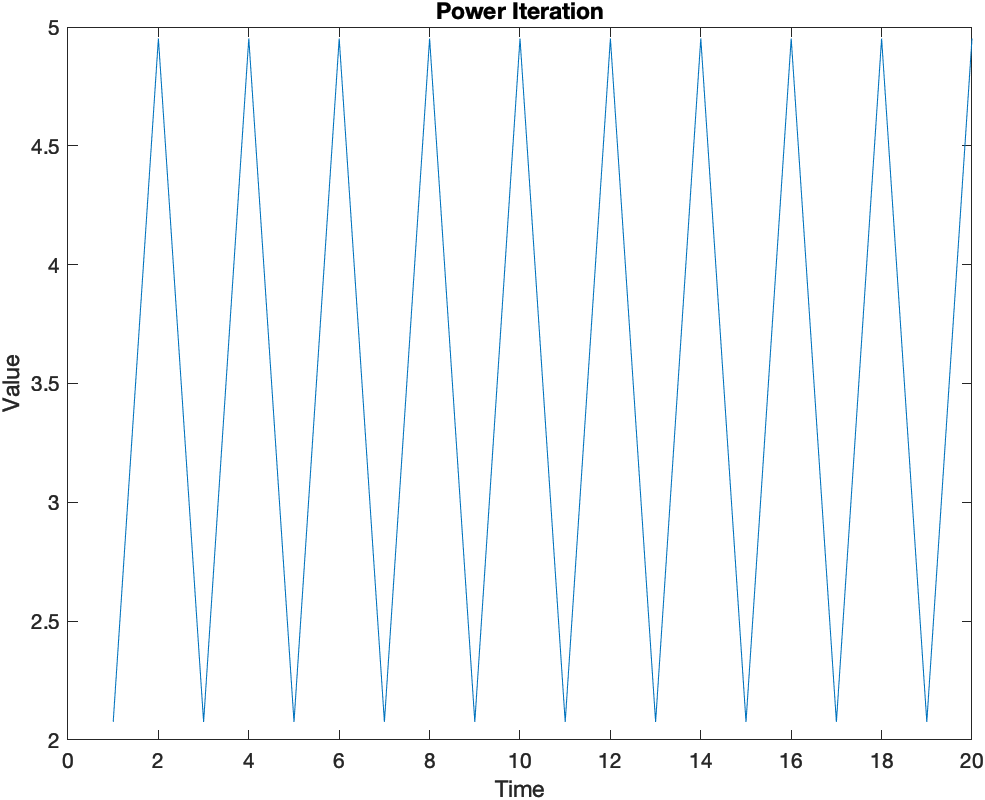
\includegraphics[width=0.4\linewidth]{p5_1.png}
	%\caption{Accuracy demo.}
\end{figure}
\begin{figure}[htbp]
	\centering
	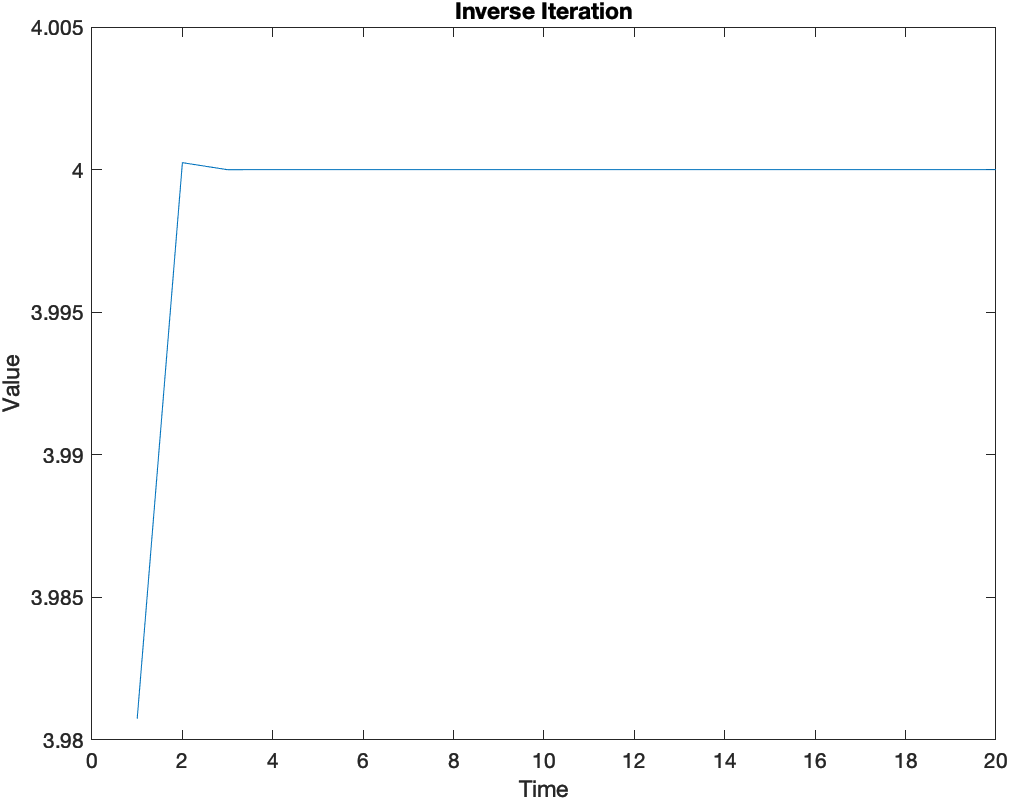
\includegraphics[width=0.4\linewidth]{p5_2.png}
	%\caption{Accuracy demo.}
\end{figure}

\newpage 
\subsection{QR itertiaon and Hessenberg QR iteration}
\noindent
\textbf{Recap.}
For $\bA \in \mathbb{C}^{n\times n}$,
consider the QR iteration (See Algorithm \ref{alg:qr_iter}) for finding all the eigenvalues and eigenvectors of $\bA$. 
\begin{algorithm}[htbp]
	\label{alg:qr_iter}
	\SetKwInOut{Input}{Input}\SetKwInOut{Output}{Output}
	\caption{QR iteration}
	\SetAlgoLined
	\Input{$\bA \in \mathbb{C}^{n\times n}$}
	\textbf{Initilization:} $\bA^{(0)} = \bA$.\\
	\For{$k= 1,\ldots, $}{
		$\bQ^{(k)}\bR^{(k)} = \bA^{(k-1)}$ \textcolor{blue}{\texttt{ \% Perform QR for $\bA^{(k-1)}$}}\\
		$\bA^{(k)} = \bR^{(k)}\bQ^{(k)}$
	}
	\Output{$\bA^{(k)}$}
\end{algorithm}
In each iteration, $\bA^{(k)}$ is similar to $\bA$ in that 
\begin{align*}
 	\bA^{(k)}
 	&  = \bR^{(k)}\bQ^{(k)} = (\bQ^{(k)})^H \bQ^{(k)}\bR^{(k)}\bQ^{(k)} = (\bQ^{(k)})^H \bA^{(k-1)}\bQ^{(k)}= \cdots \\
 	& = (\bQ^{(1)}\bQ^{(2)} \cdots \bQ^{(k)})^H \bA (\bQ^{(1)}\bQ^{(2)} \cdots \bQ^{(k)})  \Rightarrow \bA^{(k)} \text{ is similar to } \bA\,.
\end{align*}
Suppose the Schur decomposition of $\bA$ is $\bA = \bU \bT \bU^H$, then under some mild assumptions, $\bA^{(k)}$ converges to $\bT$.
Therefore, we can compute all the eigenvalues of $\bA$ by taking the diagonal elements of $\bA^{(k)}$ for sufficiently large $k$.
However, each iteration requires $\bigO(n^3)$ flops to compute QR factorization which is computationally expensive.
\begin{algorithm}[htbp]
	\label{alg:hessen_qr_iter}
	\SetKwInOut{Input}{Input}\SetKwInOut{Output}{Output}
	\caption{Hessenberg QR iteration}
	\SetAlgoLined
	\Input{$\bA \in \mathbb{C}^{n\times n}$}
	\textbf{Initilization:} $\bH = \bQ^H \bA \bQ\,,\bA^{(0)} = \bH$.  \textcolor{blue}{\texttt{ \% Hessenberg reduction for $\bA$}}\\
	\For{$k= 1,\ldots, $}{
		$\bQ^{(k)}\bR^{(k)} = \bA^{(k-1)}$ \textcolor{blue}{\texttt{ \% Perform QR for $\bA^{(k-1)}$ using Givens QR}}\\
		$\bA^{(k)} = \bR^{(k)}\bQ^{(k)}$ \textcolor{blue}{\texttt{ \% Matrix computation}}
	}
	\Output{$\bA^{(k)}$}
\end{algorithm}
One possible solution is: first perform similarity transform $\bA$ to an upper Hessenberg form (Step 1 in Algorithm \ref{alg:hessen_qr_iter}), then perform QR iteration (Algorithm \ref{alg:qr_iter}) over new $\bA^{(0)} = \bH$.
By using Givens rotations, the QR step only takes $\bigO(n^2)$ flops. 

\clearpage
\textbf{Problem 6.}
\textcolor{blue}{(15 points +10 points)}

\noindent
\begin{enumerate}
    \item Complete the Algorithm \ref{alg:hessen_qr_step} (corresponding to the step 3-4 of Algrorithm \ref{alg:hessen_qr_iter} ) first \textcolor{blue}{(7 points)}, then
show \textbf{the detailed derivation} of the computational complexity of in Algorithm \ref{alg:hessen_qr_step} ($\bigO(n^2)$). \textcolor{blue}{(8 points)}
(Derivation is for the computaional complexity of the algorithm.)

To be more specific, we can present the process of performing QR for $\bA^{(k)}$ using Givens rotations as:
\begin{enumerate}
\item[(a)] First, overwrite $\bA^{(k)}$ with upper-triangular $\bR^{(k)}$
\[
\bA^{(k)} = (\bG_{m}^H \bG_{m-1}^H \cdots \bG_{1}^H) \bA^{(k)} = \bR^{(k)}\,,
\]
where $\bG_{1},\ldots,\bG_{m}$ is a sequence of Givens rotations for some $m$ (In your algorithm, you need to clearly specify what $\bG_i$ is), and $\bR^{(k)}=\bG_1 \cdots \bG_{m}$.
\item[(b)] Perform matrix multiplication such that $\bA^{(k)}$ is of Hessenberg form,
\[
\bA^{(k)} = \bR^{(k)}\bQ^{(k)} = \bA^{(k)}\bG_1 \cdots \bG_{m}\,.
\]
\end{enumerate}
\item 
\textcolor{blue}{\textbf{(Bouns Problem})}
\textbf{Implicit QR iteration}

Another way to implement step 3-4 in Algorithm \ref{alg:hessen_qr_iter} is through \textit{implicit QR iteration}.
The idea is as follows, for $\bA^{(0)}\in \mathbb{R}^{n\times n}$ which is of Hessenberg form,
\begin{enumerate}
    \item[(a)] First, compute a Givens rotation $\bG_1$ such that $(\bG_1^{H}\bA^{(0)})_{2,1} =0$ and update $\bA^{(1)}  = \bG_1^{H} \bA^{(0)} \bG_1$. However, the entry $\bA^{(1)}_{3,1}$ may be nonzero (known as "bulge").
    \item[(b)] Compute another Givens rotation $\bG_2$ such that $(\bG_2\bA^{(1)})_{3,1} =0 $ (i.e., nulling out the "bulge") and update $\bA^{(2)}  = \bG_2^{H} \bA^{(1)} \bG_2$ which is analogous with step (a). Note that the entry $\bA^{(2)}_{4,2}$ will now be nonzero.
    \item[(c)] Then, we try to find $\bG_3$ such that $(\bG_3\bA^{(2)})_{4,2}=0$.
    The procedure of iterating nulling out the "bulges" to reset in a upper Hessenberg form is known as "bulge chasing".
\end{enumerate}
This algorithm \textit{implicitly} computed QR factorization at the cost of $\bigO(n^2)$, and this is why the algorithm is called the \textit{Implicit QR iteration}.
Consider a $4\times 4$ Hessenberg matrix
\[
\bA^{(0)} = \begin{bmatrix}
       1 & 2 & 3 & 4\\
       2 & 3 & 1 & 2\\
       0 & 1 & 3 & 2 \\
       0 & 0 & 2& 1
\end{bmatrix}\,.
\]
Carry out the implicit QR iteration (show the detailed derivation) (To simplify the computation, you can use \codeword{Matlab} to do the matrix multiplications. Specifically, explicitly show $\bG_i$, $\bG_i^H\bA^{(i-1)}$ and $\bA^{(i)}$ for each step but when computing the matrix multiplication such as $\bG_i^H\bA^{(i-1)}$, $\bG_i^H\bA^{(i-1)}\bG_i$, you are free to use \codeword{Matlab}. But be careful with the precision issue during the process of computing.), and observe where does the so-called "bulge" appears. \textcolor{blue}{(5 points: including the detailed derivation of the implicit QR iteration and pointing out the "bulge")}
Based on your observations, explain why the implicit QR iteration is indeed equivalent to the Algorithm \ref{alg:hessen_qr_step}. \textcolor{blue}{(5 points)}
\end{enumerate}




\begin{algorithm}[htbp]
	\label{alg:hessen_qr_step}
	\SetKwInOut{Input}{Input}\SetKwInOut{Output}{Output}
	\caption{Step 3-4 in Hessenberg QR iteration}
	\SetAlgoLined
	\Input{$\bA^{(k-1)} \in \mathbb{C}^{n\times n}$ which is of upper Hessenberg form \textcolor{blue}{\texttt{ \% corresponding to $\bA^{(k-1)}$ in step 3 of Algorithm \ref{alg:hessen_qr_iter}}}} 
	\textcolor{blue}{\texttt{ \% Perform QR for $\bA^{(k)}$ using Givens roations}}\\
	$A^{(k)} = A^{(k-1)}$\\
	\For{$j= 1,\ldots, n-1$}{
		$\theta_j = \arctan(-\frac{A^{k}(j+1,j)}{A^{k}(j,j)})$ \\
		$G_j = Givens\_Rotation(j,j+1,\theta_j)$	 \textcolor{blue}{\texttt{ \% Here we specify what $G_j$ is}}\\
		$A^{(k)}(j:j+1,j:n)=\begin{bmatrix}
			G_j(j,j) & G_j(j,j+1)\\
			G_j(j+1,j) & G_j(j+1,j+1)
		\end{bmatrix}^T A^{(k)}(j:j+1,j:n)$
	}
	\textcolor{blue}{\texttt{ \% Matrix computation}}\\
	\For{$j= 1,\ldots, n-1$}{
		$A^{(k)}(1:j+1,j:j+1)= A^{(k)}(1:j+1,j:j+1)\begin{bmatrix}
			G_j(j,j) & G_j(j,j+1)\\
			G_j(j+1,j) & G_j(j+1,j+1)
		\end{bmatrix}$
	}
	\Output{$\bA^{(k)}$ \textcolor{blue}{\texttt{ \% corresponding to $\bA^{(k)}$ in step 4 of Algorithm \ref{alg:hessen_qr_iter}}}}
\end{algorithm}


\noindent
\textbf{Solution}
\begin{enumerate}
    \item Complexity analysis:
    	\begin{itemize}
    		\item Givens rotation in first loop: $2\times square + 1 \times addition + 1\times root + 2 \times division = 6\, flops$.
    		\item Matrix computation in first loop: $2\times (n-j+1) \times (2 + 1) = 6(n-j+1)\,flops$.
    		\item Matrix computation in second loop:   $2\times (j+1) \times (2 + 1) = 6(j+1)\,flops$.
    	\end{itemize}
    Total complexity:
    \begin{align*}
    	&\sum_{j=1}^{n-1}\left(6 + 6(n-j+1) + 6(j+1)\right)\\
    	=&\sum_{j=1}^{n-1}(6n + 18)\\
    	=&6n^2 +12n-18\\
    	=&\mathcal{O}(6n^2)
    \end{align*}
    \item
    \begin{itemize}
    	\item Step1:
    		\begin{align*}
    			G_1 &= \begin{bmatrix}
    			0.4472 & -0.8944 & 0 & 0\\
    			0.8944 & 0.4472 & 0 & 0\\
    			0 & 0 & 1 & 0\\
    			0 & 0 & 0 & 1
     		\end{bmatrix}\\
     		G_1^HA^{(0)} &= \begin{bmatrix}
     			2.2361 & 3.5777 & 2.2361 & 3.5777\\
     			0 & -0.4472 & -2.2361 & -2.6833 \\
     			0 & 1 & 3  & 2\\
     			0 & 0 & 2 &1
     		\end{bmatrix}\\
     		A^{(1)} & = \begin{bmatrix}
     			4.2 & -0.4 & 2.2361 & 3.5777\\
     			-0.4 & -0.2 & -2.2361 & -2.6833\\
     			0.8944 & 0.4472 & 3 & 2 \\
     			0 & 0 & 2 & 1
     		\end{bmatrix}
    		\end{align*}
     		Bulge:
     		$$A^{(1)}(3,1) = 0.8944$$
     	\item Step2:
		 \begin{align*}
     		G_2 &= \begin{bmatrix}
     			1 & 0 & 0 & 0\\
     			0 & -0.4082 & -0.9129 & 0\\
     			0 & 0.9129 & -0.4082 & 0\\
     			0 & 0 & 0 & 1
     		\end{bmatrix}\\
     		G_2^H A^{(1)} & = \begin{bmatrix}
     			4.2 & -0.4 & 2.2361 & 3.5777\\
     			0.9798 & 0.4899 & 3.6515 & 2.9212 \\
     			0 & 0 & 0.8165 & 1.6330\\
     			0 & 0 & 2 & 1
     		\end{bmatrix}\\
     		A^{(2)} &= \begin{bmatrix}
     			4.2 & 2.2045 & -0.5477 & 3.5777 \\
     			0.9798 & 3.3133 & -1.9379 & 2.9212\\
     			0 & 0.7454 & -0.3333 & 1.6330\\
     			0 & 1.8257 & -0.8165 & 1
     		\end{bmatrix}
     	\end{align*}
     	Bulge:
     	$$A^{(2)}(4,2) = 1.8257$$
     \item Step3:
     \begin{align*}
     	G_3 &= \begin{bmatrix}
     		1 & 0 & 0 & 0\\
     		0 & 1 & 0 & 0\\
     		0 & 0 & 0.3780 & -0.9258\\
     		0 & 0 & 0.9258 & 0.3780
     	\end{bmatrix}\\
     	G_3^HA^{(2)} &= \begin{bmatrix}
     			4.2 & 2.2045 & -0.5477 & 3.5777 \\
     			0.9798 & 3.1333 & -1.9379 & 2.9212\\
     			0 & 1.9720 & -0.8819 & 1.5430\\
     			0 & 0  & 0 & -1.1339
     	\end{bmatrix}\\
     	A^{(3)} &= \begin{bmatrix}
     			4.2 & 2.2045 & 3.1053 & 1.8593 \\
     			0.9798 & 3.1333 & 1.9720 & 2.8983\\
     			0 & 1.9720 & 1.0952 & 1.3997\\
     			0 & 0  & -1.0498 & -0.4286
     	\end{bmatrix}
     \end{align*}
     \item The algorithm  \ref{alg:hessen_qr_step}  aim to keep the tridiagonal form of $A^{(k)}$, for the purpose of  reducing the time complexity of QR factorization in each iteration. By such a way, similarity will  also be hold so that eigenvalues could be found in the Schur form.\\
     	The implicit QR iteration shares the same idea, but the difference compared to the aforementioned algorithm lies in the  integration of the two steps in  algorithm \ref{alg:hessen_qr_step}. By such a combination, the bulges should be eliminated in each iteration in order to maintain the tridiagonal form. However, we observe that this subtle design gives no essential difference with algorithm  \ref{alg:hessen_qr_step}, since $A^{(k)} = G_m^H...G_1^HA^{(k-1)}G_1...G_m = Q^HA^{(k-1)}Q$ holds still. On one hand, this ensures the similarity between $A^{(k)}$ and $A^{(k-1)}$. On the other, tridiagonal form of $A^{(k)}$ is always maintained when output. \\Therefore, there is no essential difference between Implicit QR Iteration and Algorithm \ref{alg:hessen_qr_step}.
    \end{itemize}
\end{enumerate}

\end{document}